\documentclass[final]{beamer}
%% Possible paper sizes: a0, a0b, a1, a2, a3, a4.
%% Possible orientations: portrait, landscape
%% Font sizes can be changed using the scale option.
\usepackage[size=a0,orientation=portrait]{beamerposter}

\usetheme{gemini}
\usecolortheme{seagull}
\useinnertheme{rectangles}

% ====================
% Packages
% ====================

\usepackage[utf8]{inputenc}
\usepackage{graphicx}
\usepackage{booktabs}
\usepackage{tikz}
\usepackage{pgfplots}
\usepackage{wrapfig,lipsum}
\usepackage{cleveref}
\usepackage{subcaption}


% \usepackage{sidecap}

% ====================
% Lengths
% ====================

% If you have N columns, choose \sepwidth and \colwidth such that
% (N+1)*\sepwidth + N*\colwidth = \paperwidth
\newlength{\sepwidth}
\newlength{\colwidth}
\setlength{\sepwidth}{0.02\paperwidth}
\setlength{\colwidth}{0.47\paperwidth}
% \setlength\abovecaptionskip{-5pt}
\setlength\belowcaptionskip{-5pt}
\setlength{\headsep}{-5pt}

\newlength{\sepparagraph}
\setlength{\sepparagraph}{0.5em}

\newcommand{\separatorcolumn}{\begin{column}{\sepwidth}\end{column}}
\newcommand{\sepnewparagraph}{\vspace{\sepparagraph}}

% ====================
% Logo (optional)
% ====================

% LaTeX logo taken from https://commons.wikimedia.org/wiki/File:LaTeX_logo.svg
% use this to include logos on the left and/or right side of the header:
\logoright{\includegraphics[height=6cm]{logos/nju_logo.png}}
\logoleft{\includegraphics[height=6cm]{logos/nju_logo.png}}

% ====================
% Footer (optional)
% ====================
\footercontent{
	ICDM workshop 2024, Nanjing, China \hfill
	\insertdate \hfill
	\href{https://hhsunda.github.io/}{\texttt{hhsun@smail.nju.edu.cn}}
}

% ====================
% My own customization
% - BibLaTeX
% - Boxes with tcolorbox
% - User-defined commands
% ====================
\input{custom-defs.tex}

%% Reference Sources
\addbibresource{CFR.bib}
\addbibresource{DA_theory.bib}
\renewcommand{\pgfuseimage}[1]{\includegraphics[scale=2]{#1}}

\title{An Online Paleoclimate Data Assimilation with a Deep Learning-based Network}

\author{Haohao Sun \inst{1} \and Lili Lei \inst{1} \and Zhengyu Liu \inst{2} \and Liang Ning \inst{3} \and Zhe-Min Tan \inst{1}}

\institute[shortinst]{
    \inst{1} School of Atmospheric Sciences, Nanjing University, Nanjing \\
    \inst{2} Department of Geography, The Ohio State University, Columbus, Ohio \\
    \inst{3} School of Geography, Nanjing Normal University, Nanjing
}

\date{October 17, 2024}

\begin{document}
\setbeamercolor{background canvas}{bg=lightgray}
    \begin{frame}[t]
    	\begin{columns}
        	\begin{column}{2\colwidth+\sepwidth}
                \begin{block}{Introduction}
                    \centering
                        \begin{minipage}[t]{0.98\textwidth}
                             Paleoclimate data assimilation (PDA) combines information from climate simulations and proxy data to provide an optimal estimate of the past climate. Due to the tremendous computational cost required by lone-time simulations of an Earth system model, PDA has been traditionally performed in an offline scenario, in which priors are selected from existing paleoclimate simulations.
                            
                            \sepnewparagraph
                            
                            Currently, deep learning-based networks have been promptly developed, which are data-driven and computationally efficient after trained, and thus provide an alternative for online PDA. The deep learning-based network along with an integrated hybrid ensemble Kalman filter is proposed as an online PDA here. This online PDA can efficiently provide climate forecasts with predictive skills and effectively assimilate sparse proxy data, leading to well reconstructed surface air temperature.
                        \end{minipage}          		  		
            	\end{block}
        	\end{column}
    	\end{columns}
    
    	\begin{columns}[t]
    		\separatorcolumn		
    		\begin{column}{\colwidth}
    			
    			\begin{block}{Surrogate models}
    				\begin{itemize}
    				    \item \textbf{Linear regression model}: The linear inverse model (LIM, \cite{penland_optimal-growth_1995}) is a linear Markov process that represents the evolution of a dynamic system. The model state at $t$ mapped from the model state at $t-1$ is given by
                        \begin{equation}
                            {\bf{x}}_t^{} = {{\bf{M}}_{LIM}}{\bf{x}}_{t - 1}^{} + {\sigma _{t - 1}}
                        \end{equation}
                        where the linear operator matrix ${{\bf{M}}_{LIM}}$ is given by the regression of covariance matrices of the state vectors with time lags of 0 and 1 in the empirical orthogonal function (EOF) space.
                        \item \textbf{Deep learning-based network}: A deep learning-based network (NET) is built to map the model state at $t-1$ to that at $t$, which is a convolutional decoder-encoder (\cref{fig1}).The input and output are three-dimensional state variables, which contain augmented state variables of annual mean and six seasonal averages that are required by the proxy system models (PSMs)
                        \begin{equation}
                            {\bf{x}}_t^{} = {M_{NET}}\left( {{\bf{x}}_{t - 1}^{}} \right)   
                        \end{equation}
    				\end{itemize}
                    
                    \begin{figure}
                        \begin{minipage}[t]{0.8\textwidth}
                            \centerline{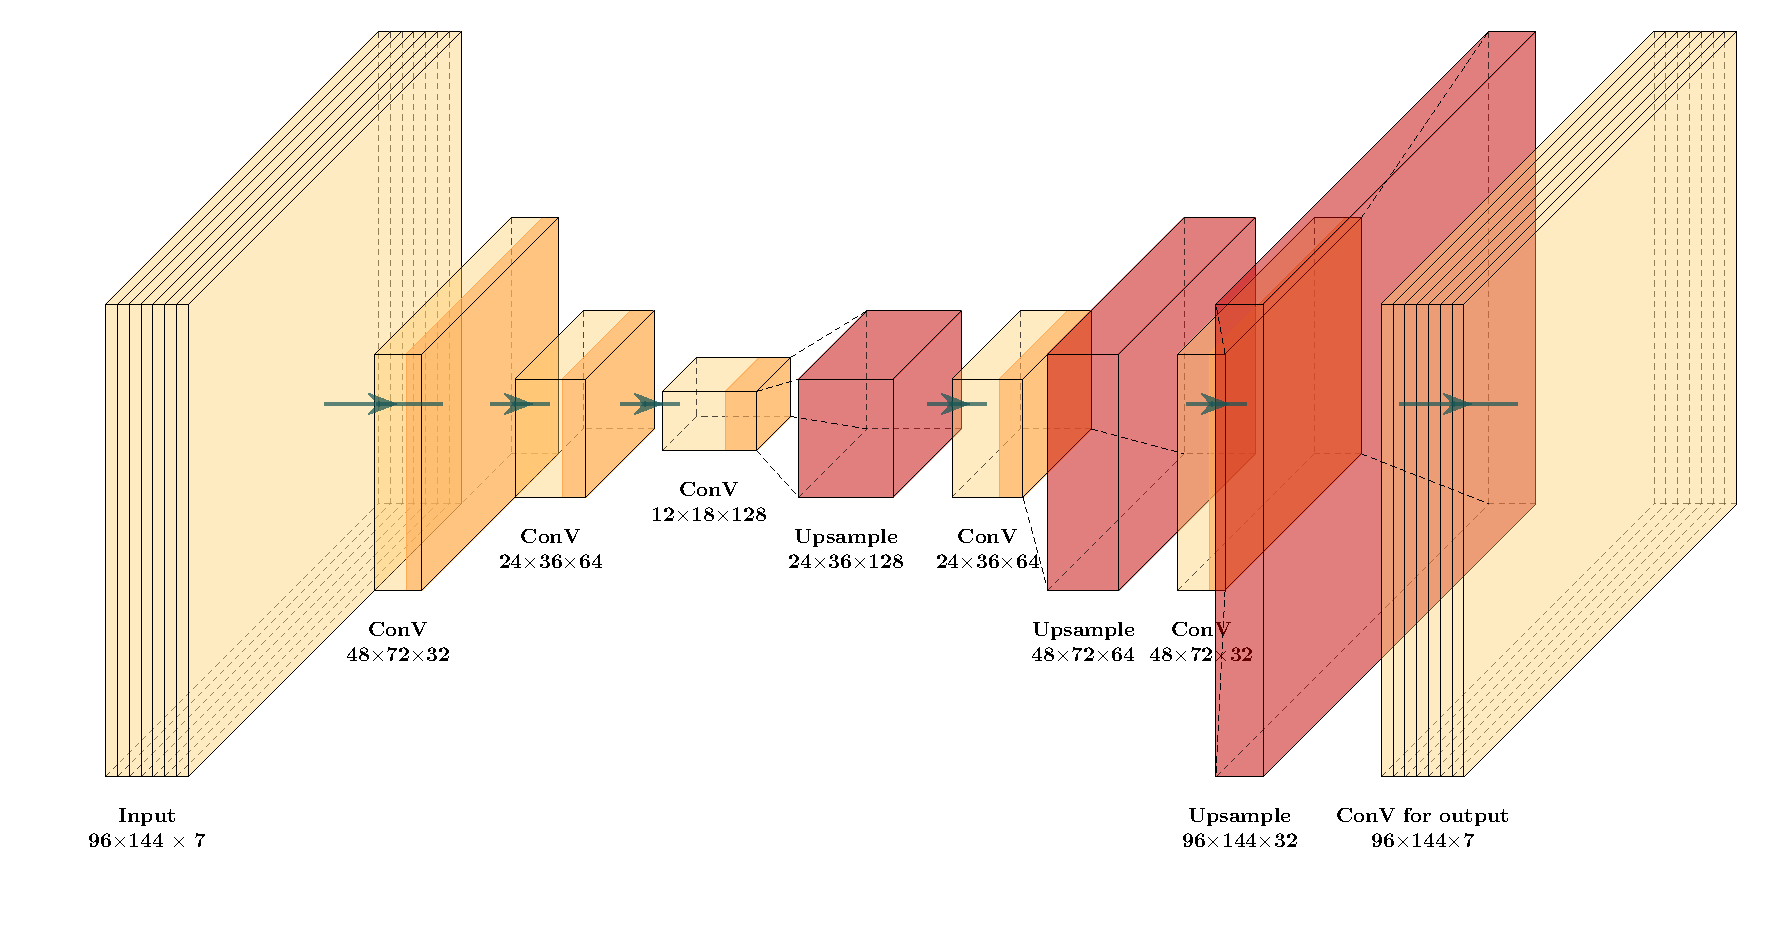
\includegraphics[width=1\textwidth]{figure/Figure1.pdf}}
                            \caption{Architecture of the convolutional decoder-encoder network. The encoder comprises one input layer, three convolutional layers (ConV), followed by three upsample-convolutional layers for the decoder. The activation layer is denoted by a darker orange shading.}\label{fig1}
                        \end{minipage}
                    \end{figure}						
    			\end{block}
    
                \begin{block}{Data assimilation methods}
                    \begin{itemize}
    					\item \textbf{Offline data assimilation}: The offline EnKF \parencite{hakim_last_2016} is used as a benchmark. Ensemble priors $\mathbf{x}^f$ are randomly sampled from a climatological simulation. The ensemble-square root filter (EnSRF), as a deterministic filter, updates the ensemble mean and ensemble perturbations separately.
                        \begin{equation}
                            {{\bf{\bar x}}^a} = {{\bf{\bar x}}^f}{\rm{ + }}{{\bf{P}}^f}{{\bf{H}}^{\rm T}}{\left[ {{\bf{H}}{{\bf{P}}^f}{{\bf{H}}^{\rm T}} + {\bf{R}}} \right]^{ - 1}}\left[ {{\bf{y}} - H\left( {{{{\bf{\bar x}}}^f}} \right)} \right]
                        \end{equation}
                        \begin{equation}
                            {\bf{x'}}_i^a = {\bf{x'}}_i^f - {{\bf{P}}^f}{{\bf{H}}^{\rm T}}{\left[ {{{\left( {\sqrt {{\bf{H}}{{\bf{P}}^f}{{\bf{H}}^{\rm T}} + {\bf{R}}} } \right)}^{ - 1}}} \right]^{\rm T}}{\left[ {\sqrt {{\bf{H}}{{\bf{P}}^f}{{\bf{H}}^{\rm T}} + {\bf{R}}}  + \sqrt {\bf{R}} } \right]^{ - 1}}\left( {{\bf{Hx'}}_i^f} \right)
                        \end{equation}
    
    					\item \textbf{Online data assimilation}: Ensemble priors $\mathbf{x}_{cyc}^f$ of online DA  are short-term forecasts based on the surrogate models. Ensemble mean and ensemble perturbations are updated separately by the hybrid background error covariances through integrated hybrid EnKF (IHEnKF, \cite{lei_integrated_2021}). The hybrid background error covariances ${\bf{P}}_{hyb}^f$ are a combination of the flow-dependent background error covariances ${\bf{P}}_{cyc}^f$ and the static background error covariances ${\bf{P}}_{climo}^f$, with weights $\alpha$ and $1-\alpha$ respectively.
                         \begin{equation}
                            {\bf{\bar x}}_{cyc}^a = {\bf{\bar x}}_{cyc}^f{\rm{ + }}{\bf{P}}_{hyb}^f{{\bf{H}}^{\rm T}}{\left[ {{\bf{HP}}_{hyb}^f{{\bf{H}}^{\rm T}} + {\bf{R}}} \right]^{ - 1}}\left[ {{\bf{y}} - H\left( {{\bf{\bar x}}_{cyc}^f} \right)} \right]
                        \end{equation}
                        \begin{equation}
                            {\bf{x'}}_{cyc,i}^a = {\bf{x'}}_{cyc,i}^f - {\bf{P}}_{hyb}^f{{\bf{H}}^{\rm T}}{\left[ {{{\left( {\sqrt {{\bf{HP}}_{hyb}^f{{\bf{H}}^{\rm T}} + {\bf{R}}} } \right)}^{ - 1}}} \right]^{\rm T}}{\left[ {\sqrt {{\bf{HP}}_{hyb}^f{{\bf{H}}^{\rm T}} + {\bf{R}}}  + \sqrt {\bf{R}} } \right]^{ - 1}}\left( {{\bf{Hx'}}_{cyc,i}^f} \right)
                        \end{equation}
                        Since the surrogate model tends to lost ensemble variances along with lead times, a blended prior is adopted \parencite{perkins_reconstructing_2017}. The selected climatological $\mathbf{x}_{\rm{climo}}^f$ or analog priors $\mathbf{x}_{\rm{analog}}^f$ can be added to the ensemble priors $\mathbf{x}_{cyc}^f$ with coefficient $\beta$:
                        \begin{equation}
                            {\bf{x}}_{cyc,i}^f = \beta M\left( {{\bf{x}}_{cyc,i}^a} \right) + \left( {1 - \beta } \right){\bf{x}}_{i}^f
                        \end{equation}
    				\end{itemize}
    			\end{block}
       
    			\begin{block}{Experimental design}			
                    \begin{itemize}
                        \item \textbf{Proxy and simulation data}: The proxy records from the PAGES 2k Consortium \parencite{pages2k_consortium_global_2017} that are temperature sensitive are assimilated, with temporal coverage of the Common Era (0-2000CE). The maximum number of proxies in 1945 CE is 554 (\cref{fig2}).
                        \item \textbf{Pseudoproxy and real proxy experiments}: Pseudoproxy data is generated by adding random error from a normal distribution to the true observed value; Real proxies from PAGES 2k are further utilized; Six different proxy networks with 50, 150, 250, 350, 450, and the full proxies are tested.  
                        \item \textbf{Evaluation metrics}: Root-mean square error (RMSE) and coefficient of efficiency (CE) are computed.        
                    \end{itemize}
    
                    \begin{figure}
                        \begin{minipage}[t]{0.8\textwidth}
                            \centerline{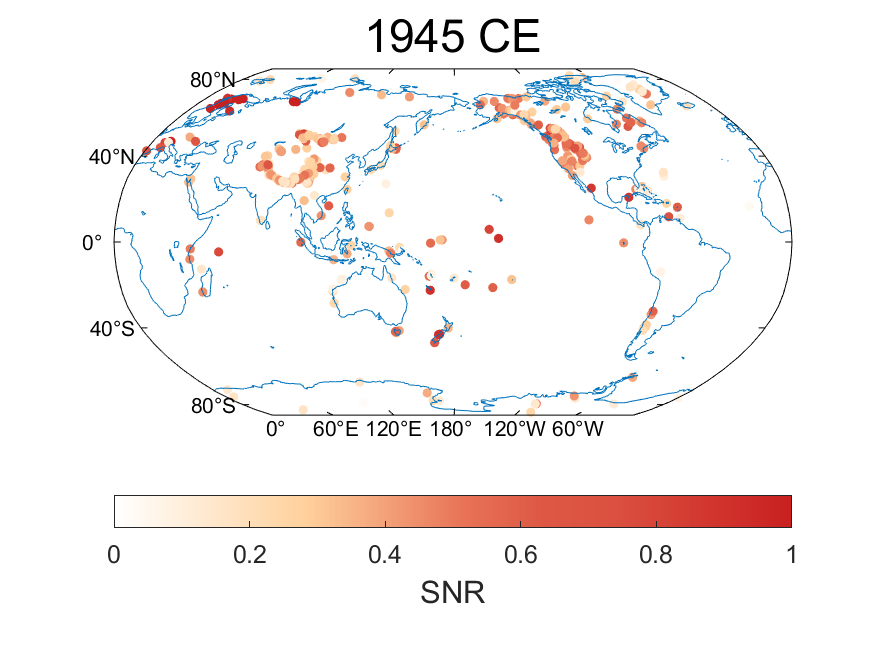
\includegraphics[width=0.625\textwidth]{figure/Figure2.png}}
                            \caption{Spatial distributions of proxy records in 1945 CE with colors indicating the signal-to-noise ratio}\label{fig2}
                        \end{minipage}
                    \end{figure}	
    			\end{block}
    
    		\end{column}	
    		\separatorcolumn	
    		\begin{column}{\colwidth}
    			
    			\begin{alertblock}{Predictive skills of surrogate models}
                    \begin{itemize}
                        \item Compared to the offline sampling, LIM has improved predictive skills within five years, and the shorter the lead time the better the predictive skill.
                        \item Compared to the LIM, the NET generally further improves the predictive skills.
                    \end{itemize}
                    \begin{figure}
                        \begin{minipage}[t]{0.8\textwidth}
                            \centerline{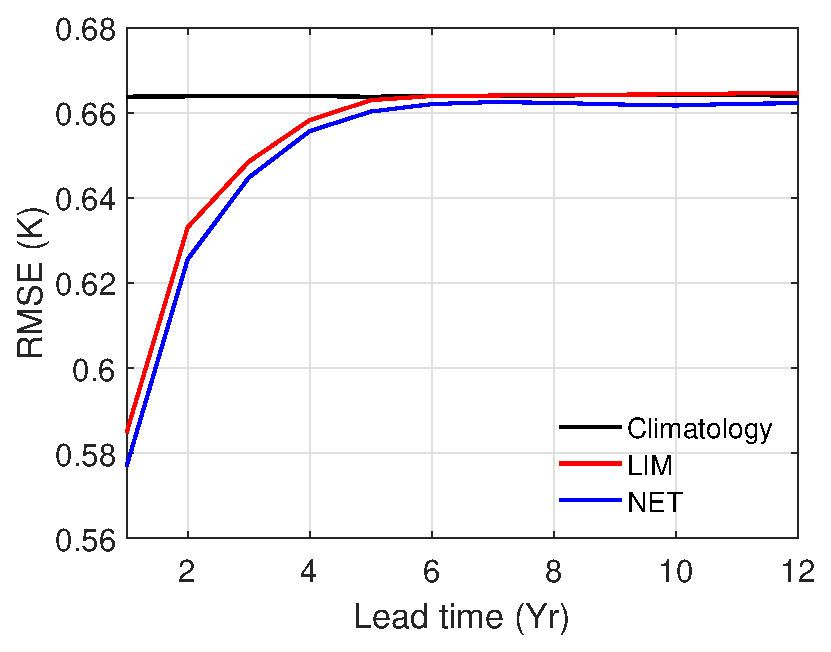
\includegraphics[width=0.49\textwidth]{figure/Figure3.eps}}
                            \caption{Spatially and temporally averaged RMSEs for climatology, LIM, and NET at various forecast lead times (years)}\label{fig3}
                        \end{minipage}
                    \end{figure}	
    			\end{alertblock}
    
    			\begin{alertblock}{Results from pseudoproxy experiments}
                    \begin{itemize}            
                        \item Exp\_LIM and Exp\_NET have larger CEs than Exp\_OFF, which indicates improved reconstruction skills from the online DA with surrogate models than the offline DA.
                        \item  Compared to Exp\_LIM, Exp\_NET obtains larger CEs of priors and posteriors, the improved predictive skills contributed by the NET than the LIM are beneficial for online DA.
                        \item  The differences between Exp\_LIM and Exp\_NET are enlarged with sparse proxy data.
                    \end{itemize}
                    \begin{figure}
                        \begin{minipage}[t]{0.8\textwidth}
                            \centering
                            \begin{minipage}[t]{0.49\textwidth}
                                \begin{tikzpicture}
                                    \node[anchor=north west] at (0,0) {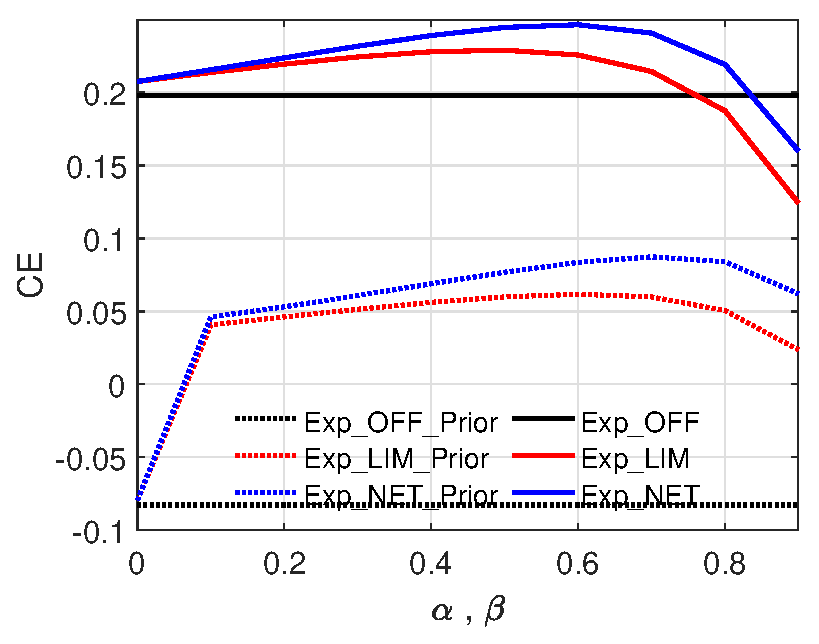
\includegraphics[width=\textwidth]{figure/Figure4a.eps}};   
                                    \node[anchor=north west, fill=white, text=black, font=\bfseries] at (0.01, 0.01) {(a)};
                                \end{tikzpicture}
                            \end{minipage}
                            \begin{minipage}[t]{0.49\textwidth}
                                \begin{tikzpicture}
                                    \node[anchor=north west] at (0,0) {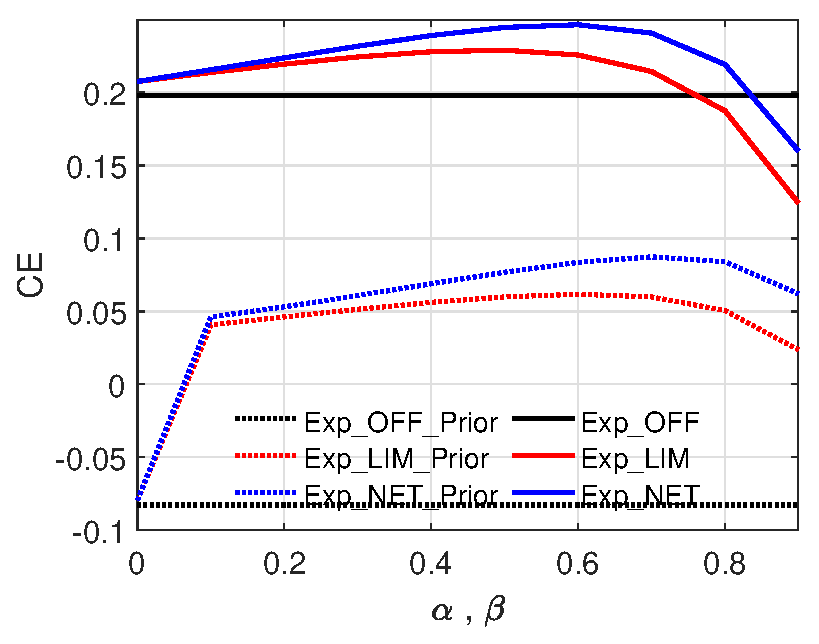
\includegraphics[width=\textwidth]{figure/Figure4a.eps}};   
                                    \node[anchor=north west, fill=white, text=black, font=\bfseries] at (0.01, 0.01) {(b)};
                                \end{tikzpicture}
                            \end{minipage}    
                            \caption{Area-weighted global averaged CEs for Exp\_OFF, Exp\_LIM, and Exp\_NET with varying hybrid weights / blending weights, assimilating a proxy network with (a) 150 pseudoproxies and (b) full pseudoproxies.}\label{fig4}
                        \end{minipage}
                    \end{figure}
    			\end{alertblock}
    
    			\begin{alertblock}{Results from real proxy experiments}
                    \begin{itemize}
                        \item When a full set of proxy data is used, offline DA and online DA with either LIM or NET have similar GMT reconstructions, which are mainly forced by the proxy information.
                        \item When a limited set of proxies is used, Exp\_OFF has reduced GMT variability than Exp\_LIM and Exp\_NETANA.   
                        \item Compared to Exp\_LIM with linear predictive skills obtained by the LIM, Exp\_NETANA benefits from retaining nonlinear dynamics provided by the NET and further incorporating analog climatological ensembles, which leads to improved GMT reconstruction even with limited proxies.
                    \end{itemize}
                    \begin{figure}
                        \begin{minipage}[t]{0.8\textwidth}
                            \centering
                            \begin{minipage}[t]{0.49\textwidth}
                                \begin{tikzpicture}
                                    \node[anchor=north west] at (0,0) {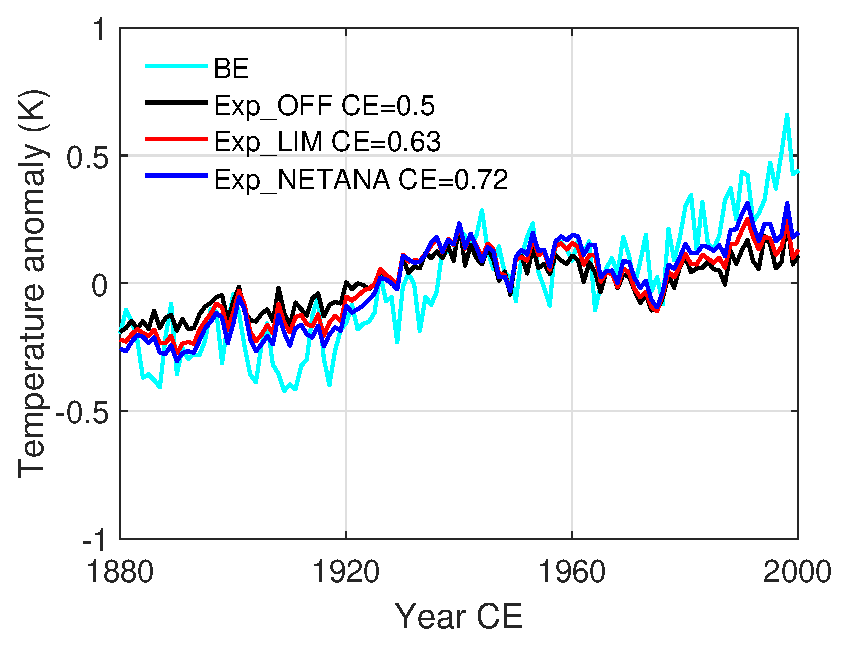
\includegraphics[width=\textwidth]{figure/Figure5a.eps}};   
                                    \node[anchor=north west, fill=white, text=black, font=\bfseries] at (0.01, 0.01) {(a)};
                                \end{tikzpicture}
                            \end{minipage}
                            \begin{minipage}[t]{0.49\textwidth}
                                \begin{tikzpicture}
                                    \node[anchor=north west] at (0,0) {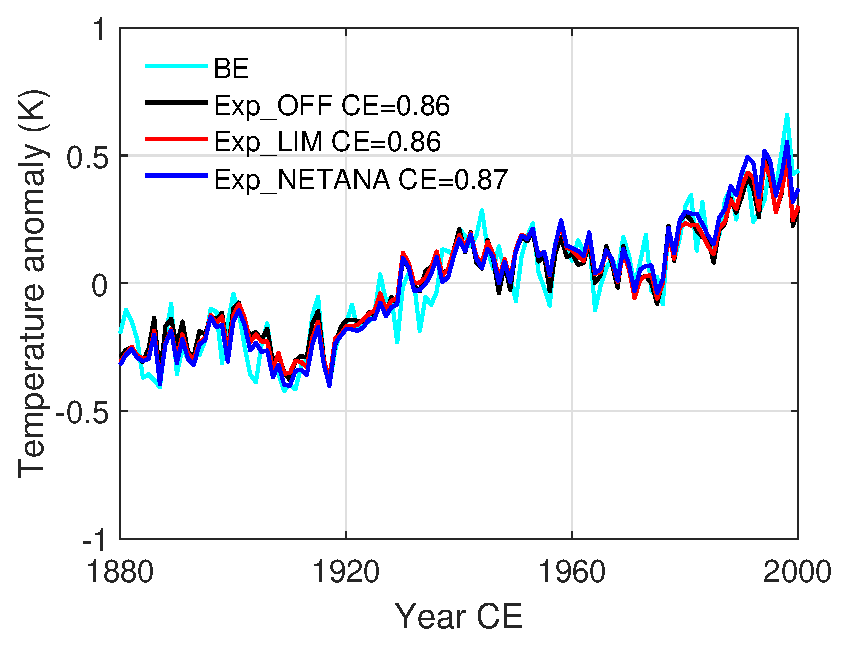
\includegraphics[width=\textwidth]{figure/Figure5b.eps}};   
                                    \node[anchor=north west, fill=white, text=black, font=\bfseries] at (0.01, 0.01) {(b)};
                                \end{tikzpicture}
                            \end{minipage}    
                            \caption{The reconstruction of GMTs over the instrumental period for Exp\_OFF, Exp\_LIM, and Exp\_NETANA given a hybrid weight / blending weight of 0.7, assimilating a proxy network with (a) 150 proxies and (b) full proxies.}
                            \label{fig5}
                        \end{minipage}
                    \end{figure}
                    \begin{itemize}
                        \item The GMT reconstruction provided by the online PDA has smaller spread but more consistent error statistics than those provided by the online PDA with LIM and offline PDA, during the early period with limited proxy data.
                    \end{itemize}
                    \begin{figure}
                        \begin{minipage}[t]{0.8\textwidth}
                            \centerline{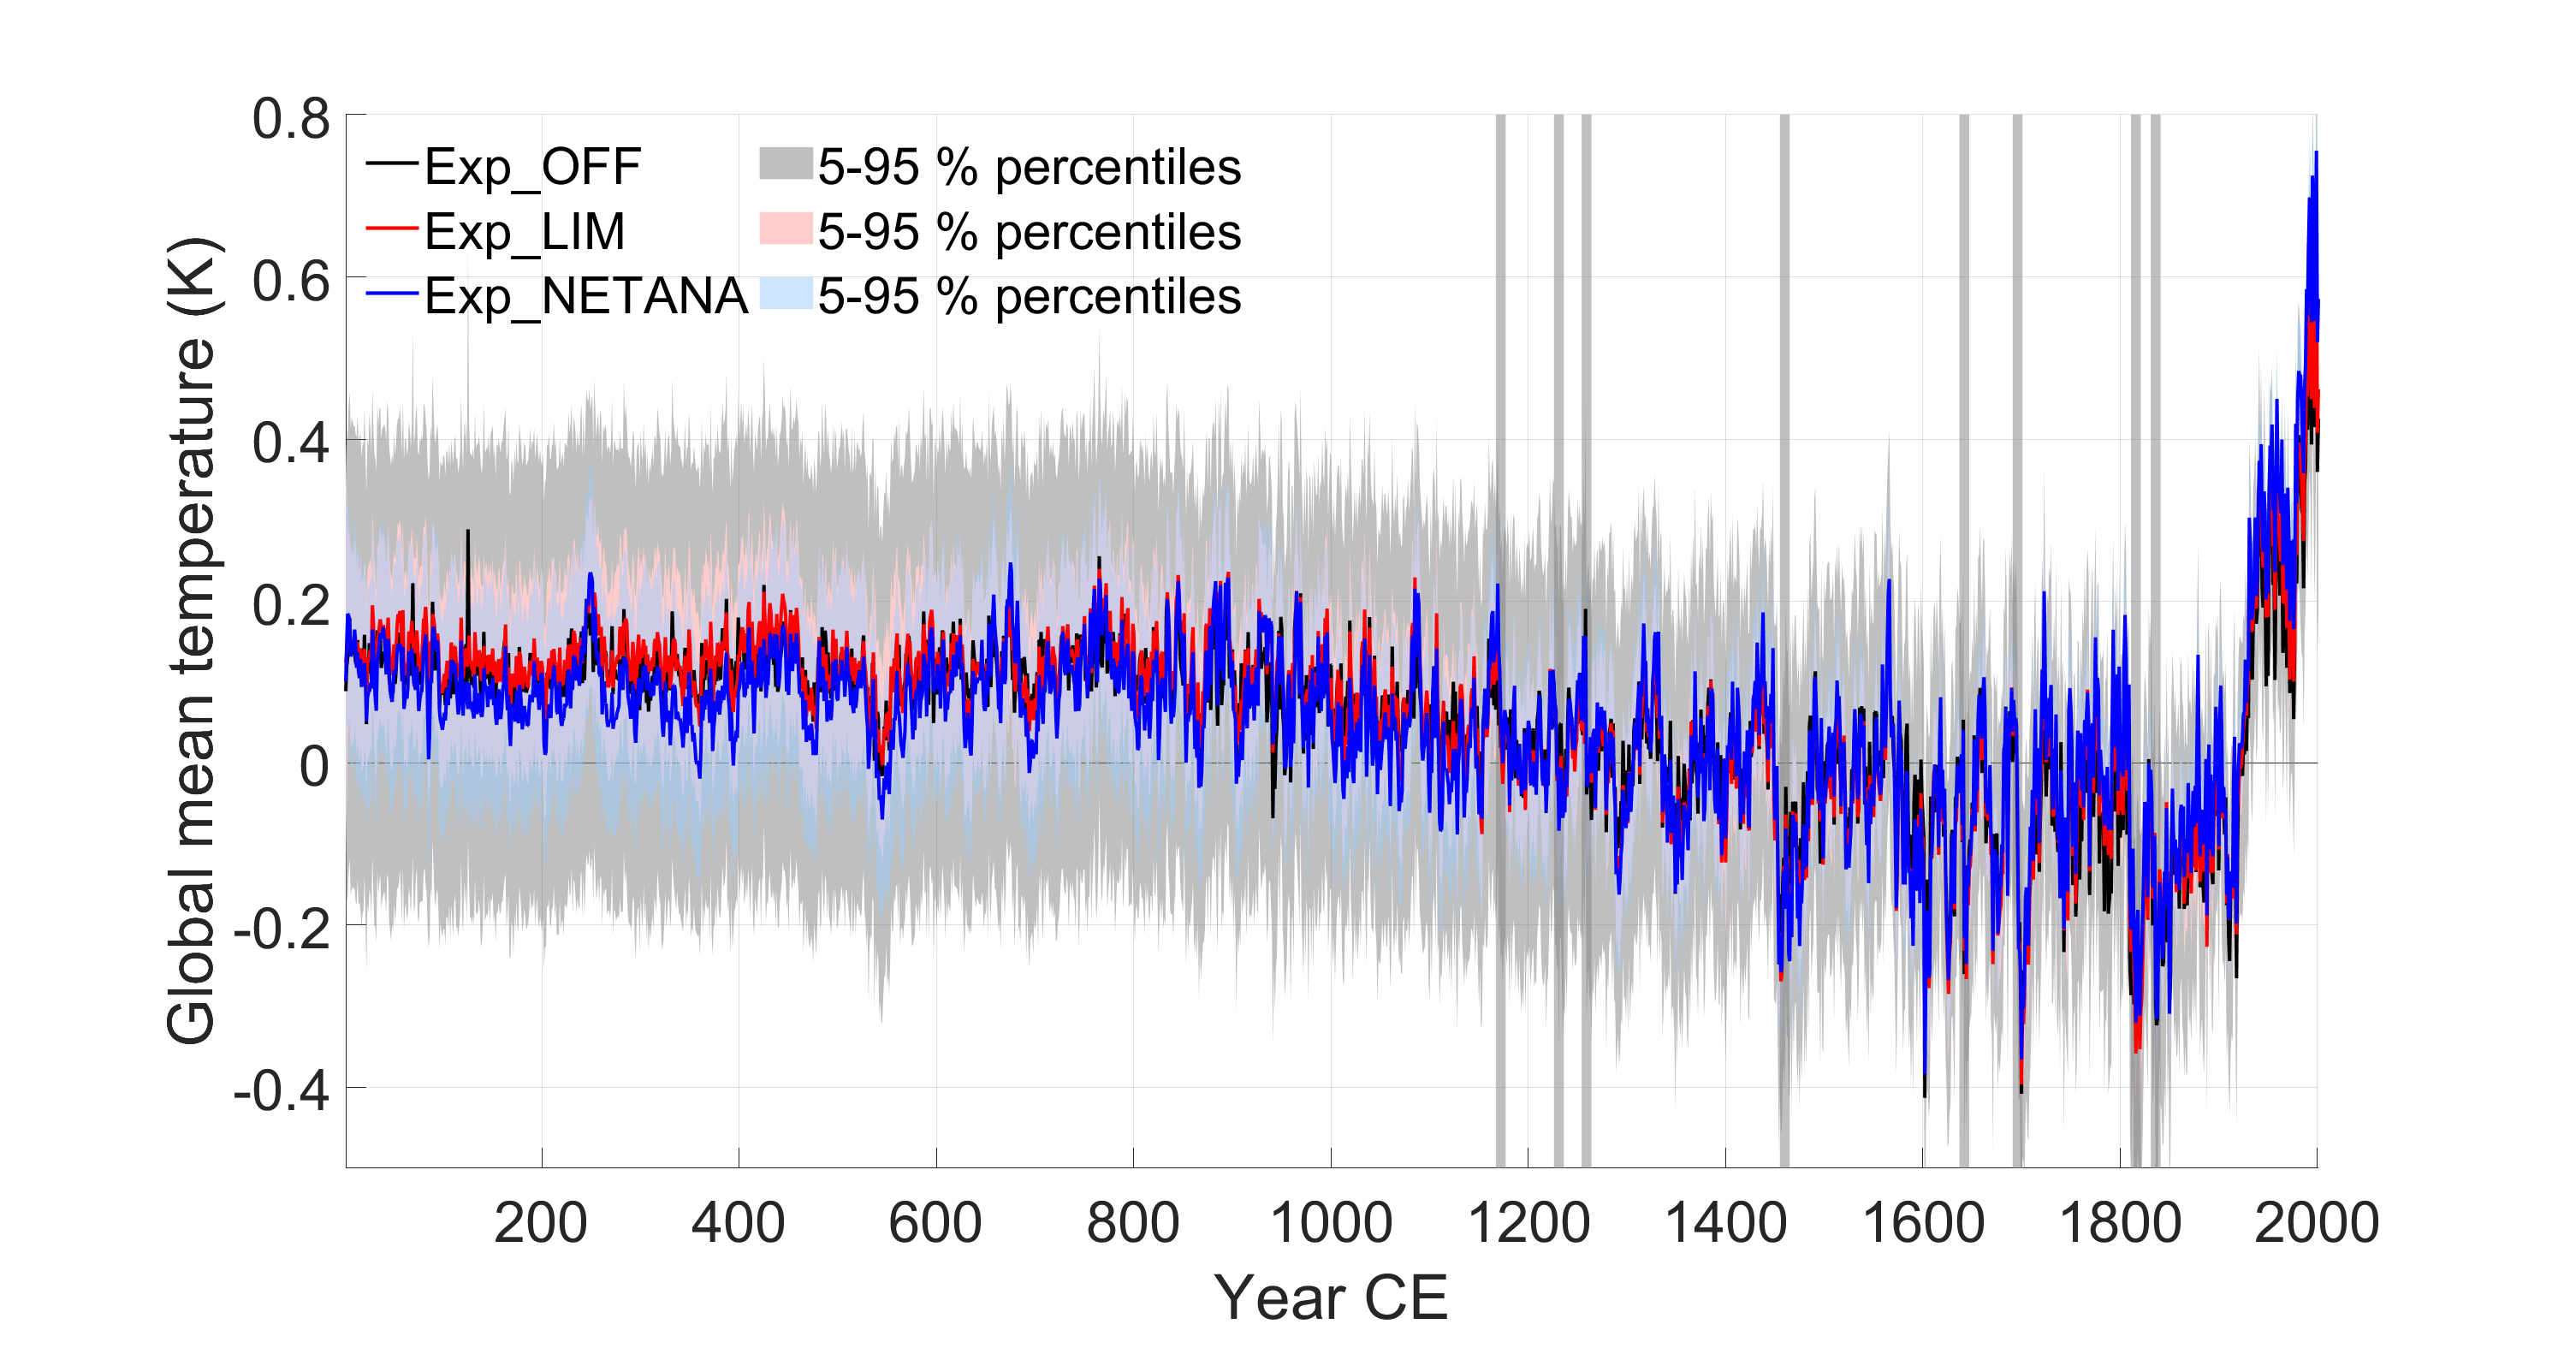
\includegraphics[width=1\textwidth]{figure/Figure6.eps}}
                            \caption{The reconstruction of GMTs over the Common Era for Exp\_OFF, Exp\_LIM, and Exp\_NETANA, given a hybrid weight / blending weight of 0.7, assimilating a proxy network with full proxies. The vertical grey lines denote the volcanic eruption years.}\label{fig6}
                        \end{minipage}
                    \end{figure}
    			\end{alertblock}
    			
    		\end{column}		
    		\separatorcolumn
    	\end{columns}
    \end{frame}
\end{document}